\begin{figure}[htbp]
	% Partly taken from http://www.texample.net/tikz/examples/convolution-of-two-functions/
	\centering
	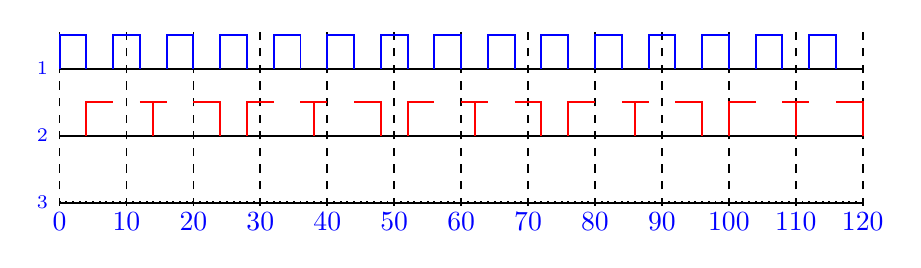
\begin{tikzpicture}[
		scale=0.085,
		line width=0.25mm,
		every node/.style={scale=1, text=blue},
		major tick/.style={semithick, dashed},
		x tick label/.style={anchor=north, minimum width=5mm},
		task1/.style={blue},
		task2/.style={red},
		task3/.style={green},
		desc/.style={anchor=east}
		]


	% Task 3
	\draw (0, 0) -- (120, 0);
	\node[desc] at (0, 0) {$\uptau_3$};
	
	% Task 2
	\draw (0, 10) -- (120, 10);
	\node[desc] at (0, 10) {$\uptau_2$};	

	% Task 1
	\draw (0, 20) -- (120, 20);
	\node[desc] at (0, 20) {$\uptau_1$};	

	
	% Small ticks
	\foreach \x in {0, 1,...,120}{
		\draw (\x, -0.25) -- (\x, 0.25);
	}
	
	% Major ticks with label
	\foreach \x/\label in {0, 10,...,120}{
		\node[x tick label] at (\x, 0) {$\label$}; 		
		\draw[major tick] (\x, -0.5) -- (\x, 26);
	}
	
	% Draw all
	\foreach \x in {0, 24,...,100}{
		\draw[task1] (\x, 20) -- (\x, 25) -- (\x+4, 25) -- (\x+4, 20);
		\draw[task2] (\x+4, 10) -- (\x+4, 15) -- (\x+8, 15);
		\draw[task1] (\x+8, 20) -- (\x+8, 25) -- (\x+12, 25) -- (\x+12, 20);
		\draw[task2] (\x+12, 15) -- (\x+14, 15) -- (\x+14, 10);
		\draw[task2] (\x+14, 10) -- (\x+14, 15) -- (\x+16, 15);
		\draw[task1] (\x+16, 20) -- (\x+16, 25) -- (\x+20, 25) -- (\x+20, 20);
		\draw[task2] (\x+20, 15) -- (\x+24, 15) -- (\x+24, 10);
	}

%	\draw[task1] (0, 10) --  (0, 15) --  (4, 15) -- (4, 10);	

		
	\end{tikzpicture}
%	\caption{Ablaufübersicht}
\end{figure} 